\documentclass[11pt]{article}
\usepackage[margin=2.5cm]{geometry}
\usepackage{amsmath,amssymb,amsthm}
\usepackage{booktabs}
\usepackage{graphicx}
\usepackage{xurl}
\usepackage[hidelinks]{hyperref}

\newtheorem{theorem}{Theorem}
\newtheorem{proposition}[theorem]{Proposition}
\newtheorem{lemma}[theorem]{Lemma}
\newtheorem{corollary}[theorem]{Corollary}
\theoremstyle{remark}
\newtheorem{remark}[theorem]{Remark}

\newcommand{\Tr}{\operatorname{Tr}}
\newcommand{\Q}{\mathbb{Q}}
\newcommand{\Z}{\mathbb{Z}}

\title{Pisot units and the third manuscript on page 343\\ of Ramanujan's Lost Notebook}
\author{Otakhon U. Kenjaev\\ \small Independent researcher, Khorezm, Uzbekistan\\
\small ORCID \href{https://orcid.org/0009-0009-3566-9285}{0009-0009-3566-9285}}
\date{September 2026}

\begin{document}
\maketitle

\begin{abstract}
Page 343 of Ramanujan's Lost Notebook claims that $a^m b^n\theta$ is close to an integer, with an explicit error term, where
$\theta=2^{1/5}$, $a=1/(\theta-1)$ and $b=\sqrt5/(1+\theta^2)^{5/2}$; a second claim of the same kind concerns $2^{1/7}$. Andrews and
Berndt (Lost Notebook, Part~IV, Section~7.4) were unable to give these claims a meaning and wrote that they are wrong. We show that
$a=1+\theta+\theta^2+\theta^3+\theta^4$ and $b=1-\theta-\theta^2+\theta^4$ are units of $\Z[\theta]$, that each factor of Ramanujan's
error term is the modulus of a Galois conjugate of $a^mb^n$, and that the integer is $\Tr(a^mb^n\theta)$. This gives a proof of the
first claim with the explicit bound $2\theta(|\sigma_1(a^mb^n)|+|\sigma_2(a^mb^n)|)$; the constant $2\theta$ is sharp, and the bound
tends to $0$ exactly along sequences with $m-6.0114\,n\to\infty$. We explain the change between the two cases: $1/(2^{1/p}-1)$ is a Pisot number if and only
if $p\le6$. For $2^{1/7}$ the printed error term does not match the conjugates in three places; after correcting them the claim holds
on an explicit cone of exponents. All statements are accompanied by a verification script.
\end{abstract}

\noindent\textit{2020 Mathematics Subject Classification:} 11J68, 11R06, 11R27, 01A60.\\
\textit{Keywords:} Ramanujan's lost notebook, Pisot numbers, units, Diophantine approximation, pure quintic field.

\section{Introduction}
The last section of Chapter~7 of \cite{AB4} reproduces page~343 of \cite{LN}. With $\theta=2^{1/5}$,
\begin{equation}\label{eq:ab}
a=\frac1{2^{1/5}-1},\qquad b=\frac{\sqrt5}{(1+4^{1/5})^{5/2}},\qquad a^mb^n\theta=p_{m,n}+\epsilon_{m,n},\quad
-\tfrac12<\epsilon_{m,n}<\tfrac12,\ p_{m,n}\in\Z,
\end{equation}
Ramanujan states
\begin{equation}\label{eq:741}
\epsilon_{m,n}=O\!\left(\frac{5^{n/2}}{\bigl(4^{1/5}-2\cdot2^{1/5}\cos\frac{2\pi s}5+1\bigr)^{m/2}
\bigl(16^{1/5}+2\cdot4^{1/5}\cos\frac{4\pi s}5+1\bigr)^{5n/4}}\right),
\end{equation}
``where $s$ is the most unfavorable of the integers 1, 2, 3, 4'' (this is (7.4.1) of \cite{AB4}). A second claim, (7.4.2), concerns
$\theta=2^{1/7}$ and three numbers $a,b,c$ (Section~\ref{sec:seven}). Andrews and Berndt tabulate $\epsilon_{m,n}$ for $m,n\le10$ and
conclude: ``We have been unable to provide meaning to the third manuscript, which is on page 343. Its claims are wrong, and so it
remains a challenge to determine whether something meaningful can be ascertained'' \cite[p.~164]{AB4}. They also ask why
Ramanujan lists four values of $s$ and what role $\theta$ plays, and they observe that a meaningful statement would need $m$ and
$n$ to tend to infinity along special sequences \cite[p.~180]{AB4}.

\medskip\noindent\textbf{Contribution.} The phenomenon is that of Pisot numbers \cite{Thue,Hardy,Pisot,BDGPS}: if $\alpha$ is a real
algebraic integer whose other conjugates lie inside the unit circle, then $\alpha^m$ is close to the integer $\Tr\alpha^m$. We do not
claim a new method. What is new is the identification of Ramanujan's data: $a,b$ are units (Section~\ref{sec:five}), his error
factors are exactly the conjugate moduli (Lemma~\ref{lem:factors}), and the four values of $s$ are the four non-real embeddings.
This answers the questions above and gives Theorem~\ref{thm:main}, a sharpness statement (Proposition~\ref{prop:sharp}), an
explanation of the two cases $5$ and $7$ (Lemma~\ref{lem:pisot}), and a corrected form of (7.4.2) (Theorem~\ref{thm:seven}).

\medskip\noindent\textbf{Prior literature.} The first manuscript of Chapter~7 (pages 262--265) was treated by Berndt and Kim
\cite{BK}. We found no treatment of page~343 in zbMATH Open (eight queries and all 53 documents citing \cite{AB4}), OpenAlex or
Google Scholar (September 2026).

\section{The quintic case}\label{sec:five}
Let $K=\Q(\theta)$, $\theta=2^{1/5}$, $\zeta=e^{2\pi i/5}$, and let $\sigma_s$ ($0\le s\le4$) be the embedding with
$\sigma_s(\theta)=\theta\zeta^s$. Then $\sigma_0$ is real, $\sigma_4=\overline{\sigma_1}$ and $\sigma_3=\overline{\sigma_2}$.

\begin{lemma}\label{lem:units}
In $\Z[\theta]$ we have $a=1+\theta+\theta^2+\theta^3+\theta^4$ and $b=1-\theta-\theta^2+\theta^4$, and
\[
a(\theta-1)=1,\qquad b^2(1+\theta^2)^5=5,\qquad N_{K/\Q}(a)=N_{K/\Q}(b)=1,\qquad N_{K/\Q}(1+\theta^2)=5 .
\]
The minimal polynomials are $x^5-5x^4-10x^3-10x^2-5x-1$ for $a$ and $x^5-5x^4+20x^3-10x^2+5x-1$ for $b$.
\end{lemma}

\begin{proof}
$(\theta-1)(1+\theta+\dots+\theta^4)=\theta^5-1=1$. Reducing $(1-\theta-\theta^2+\theta^4)^2(1+\theta^2)^5$ modulo
$\theta^5-2$ gives $5$. Since $b>0$ and $b^2=5/(1+\theta^2)^5$, $b$ is Ramanujan's number. The norms are resultants with $x^5-2$.
\end{proof}

Thus $5$ is totally ramified, $5=(1+\theta^2)^5b^2$, and $b$ is the unit attached to this factorization. The regulator of $\{a,b\}$
is $4.83493544801521$, equal to the regulator of $K$ listed in the LMFDB (field 5.1.50000.1, class number 1) \cite{LMFDB}; hence
$\{a,b\}$ is a system of fundamental units.

\begin{lemma}\label{lem:factors}
For $1\le s\le4$,
\[
|\sigma_s(a)|^{-2}=4^{1/5}-2\cdot2^{1/5}\cos\tfrac{2\pi s}5+1,\qquad
|\sigma_s(b)|^{2}=\frac5{\bigl(16^{1/5}+2\cdot4^{1/5}\cos\frac{4\pi s}5+1\bigr)^{5/2}} .
\]
Hence the expression inside $O(\cdot)$ in \eqref{eq:741} equals $|\sigma_s(a^mb^n)|$.
\end{lemma}

\begin{proof}
$|\sigma_s(a)|^{-2}=|\theta\zeta^s-1|^2=\theta^2-2\theta\cos(2\pi s/5)+1$, and by Lemma~\ref{lem:units}
$|\sigma_s(b)|^2=5/|1+\theta^2\zeta^{2s}|^5$ with $|1+\theta^2\zeta^{2s}|^2=\theta^4+2\theta^2\cos(4\pi s/5)+1$.
\end{proof}

Numerically $|\sigma_1(a)|=0.7882149$, $|\sigma_2(a)|=0.4892248$, $|\sigma_1(b)|=4.1813005$, $|\sigma_2(b)|=0.4578160$. In
particular $a$ is a Pisot unit. Put $A_s(m,n)=|\sigma_s(a)|^m|\sigma_s(b)|^n$.

\begin{theorem}\label{thm:main}
For all integers $m,n\ge0$ let $p_{m,n}=\Tr_{K/\Q}(a^mb^n\theta)$. Then $p_{m,n}\in5\Z$, and $\epsilon_{m,n}=a^mb^n\theta-p_{m,n}$ satisfies
\[
\epsilon_{m,n}=-\sum_{s=1}^4\sigma_s(a^mb^n\theta),\qquad |\epsilon_{m,n}|\le2\theta\bigl(A_1(m,n)+A_2(m,n)\bigr)\le4\theta\max_{1\le s\le4}A_s(m,n).
\]
Consequently \eqref{eq:741} holds for all $m,n$ (with $p_{m,n}$ the trace), with implied constant $4\theta$ and with $s$ the index maximizing Ramanujan's
error factor. Along a sequence with $m+n\to\infty$ the bound tends to $0$ if and only if $m-\kappa n\to\infty$, where
$\kappa=\log|\sigma_1(b)|/(-\log|\sigma_1(a)|)=6.0114084$; along such a sequence $p_{m,n}$ is eventually the integer nearest to
$a^mb^n\theta$, as in \eqref{eq:ab}.
\end{theorem}

\begin{proof}
$a^mb^n\theta\in\Z[\theta]$, and $\Tr(\theta^k)=0$ for $1\le k\le4$, $\Tr(1)=5$; so $p_{m,n}$ is five times the constant coordinate.
The trace is the sum of the five embeddings, which gives the formula for $\epsilon_{m,n}$; the conjugate pairs contribute
$2\operatorname{Re}\sigma_s(a^mb^n\theta)$ with $|\sigma_s(\theta)|=\theta$. Since $|\sigma_2(a)|,|\sigma_2(b)|<1$, $A_2\to0$ as
$m+n\to\infty$, while $\log A_1=m\log|\sigma_1(a)|+n\log|\sigma_1(b)|$.
\end{proof}

For $n=0$ the bound is below $\tfrac12$ for $m\ge7$; direct computation shows that $p_{m,0}$ is the nearest integer also for $m=4,6$,
but not for $m\in\{0,1,2,3,5\}$ (for instance $p_{2,0}=50$ while $a^2\theta=51.951$). The table in \cite[p.~181]{AB4} stops at $m=10$,
where the bound $2\theta(A_1+A_2)$ is still $0.2145$; this is why the remainders there looked random. The sequences along which the
claim is meaningful, asked for in \cite[p.~180]{AB4}, are exactly those with $m-\kappa n\to\infty$.

\begin{remark}\label{rem:theta}
The factor $\theta$ plays no special role: for any $\gamma\in\Z[\theta]$ the same proof gives
$|a^mb^n\gamma-\Tr(a^mb^n\gamma)|\le2\sum_{s=1,2}|\sigma_s(\gamma)|A_s(m,n)$. For $\gamma=\theta$ all conjugates have the same
modulus $\theta$, which is why Ramanujan's error term contains no factor depending on $\gamma$. This answers the question about
the role of $\theta$ in \cite[p.~180]{AB4}.
\end{remark}

\begin{proposition}\label{prop:sharp}
$\limsup_{m\to\infty}|\epsilon_{m,0}|/|\sigma_1(a)|^m=2\theta$. Thus the constant $2\theta$ in Theorem~\ref{thm:main} cannot be reduced.
\end{proposition}

\begin{proof}
We have $\epsilon_{m,0}=-2\operatorname{Re}\sigma_1(a^m\theta)-2\operatorname{Re}\sigma_2(a^m\theta)$, and the second term is
$O(|\sigma_2(a)|^m)=o(|\sigma_1(a)|^m)$. Let $\varphi=\arg\sigma_1(a)$. If $\varphi/\pi$ were rational, then $\sigma_1(a)^N=\sigma_4(a)^N$ for
some $N\ge1$. The Galois group of $x^5-2$ (of order 20) acts transitively on the conjugates, so some automorphism $\tau$ maps $\sigma_1(a)$
to $a$; then $a^N=\tau(\sigma_4(a))^N$, which is impossible because $a>1$ and the right side has modulus $<1$. Hence
$\{m\varphi/2\pi\}$ is dense in $[0,1)$ and $\cos(m\varphi+\arg(\theta\zeta))$ comes arbitrarily close to $\pm1$.
\end{proof}

\section{Why five and seven}\label{sec:why}
\begin{lemma}\label{lem:pisot}
For $p\ge2$ the unit $a_p=1/(2^{1/p}-1)$ is a Pisot number if and only if $2^{1/p}>2\cos(2\pi/p)$, that is, if and only if $p\le6$.
\end{lemma}

\begin{proof}
$x^p-2$ is irreducible (Eisenstein), and the conjugates of $a_p$ other than $a_p$ are $1/(\theta\zeta_p^s-1)$, $1\le s\le p-1$. Now
$|\theta\zeta_p^s-1|^2=\theta^2-2\theta\cos(2\pi s/p)+1$ is smallest for $s=1$, and it exceeds $1$ exactly when $\theta>2\cos(2\pi/p)$. For
$p\le6$ we have $2\cos(2\pi/p)\le1<2^{1/p}$; for $p\ge7$, $2\cos(2\pi/p)\ge2\cos(2\pi/7)=1.2470>2^{1/7}\ge2^{1/p}$.
\end{proof}

The largest other conjugate of $a_p$ has modulus $0.9376$ for $p=6$ and $1.0896$ for $p=7$ (Figure~\ref{fig:boundary}). So $p=5$ is the
last odd exponent for which $a$ alone is Pisot, and $p=7$ is the first for which it is not; this is why (7.4.2) needs further units.
In both cases Ramanujan's second unit comes from the totally ramified prime above $p$: $b^2=5/(1+\theta^2)^5$ for $p=5$ and
$b=7/(\theta^3-1)^7$ for $p=7$ (for $p=3$ the analogous unit $3/(1+\theta)^3=\theta-1=1/a$ gives nothing new).

\begin{figure}[ht]
\centering
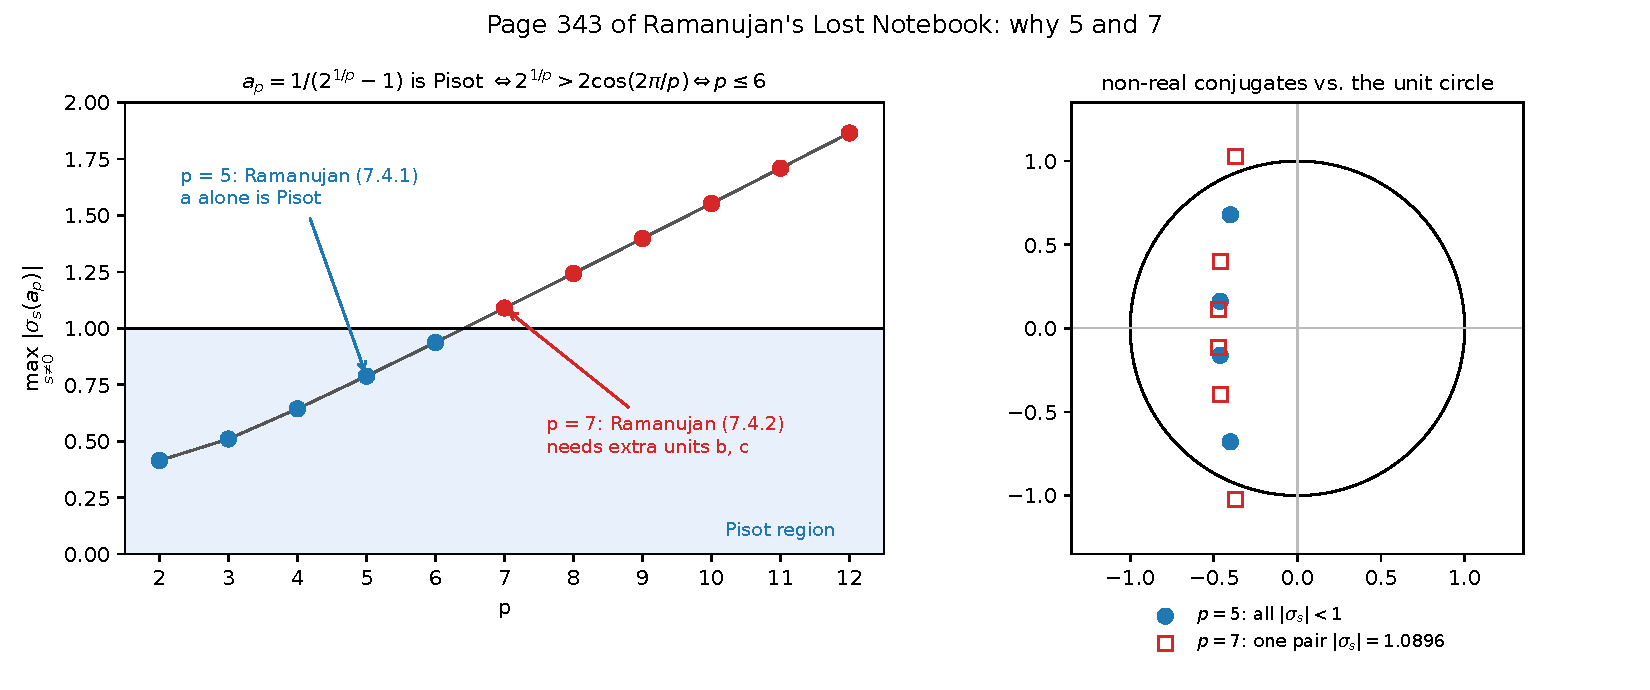
\includegraphics[width=\textwidth]{p343_boundary.pdf}
\caption{Left: the largest modulus of the other conjugates of $1/(2^{1/p}-1)$. Right: the non-real conjugates for $p=5$ and $p=7$
and the unit circle.}\label{fig:boundary}
\end{figure}

\section{The septic case}\label{sec:seven}
Let now $\theta=2^{1/7}$, $\sigma_s(\theta)=\theta e^{2\pi is/7}$, and, as on page 343,
\[
a=\frac1{\theta-1},\qquad b=\frac7{(\theta^3-1)^7},\qquad c=\frac{\theta+1}{\theta^2-\theta+1},\qquad a^\ell b^mc^n\theta=p_{\ell,m,n}+\epsilon_{\ell,m,n}.
\]
All three are units (their minimal polynomials are monic with constant term $-1$); $N(\theta^3-1)=7$ and $c=(\theta+1)^2/(\theta^3+1)$.
The error term printed as (7.4.2) in \cite{AB4} is
\[
O\!\left(\frac{7^m\bigl(\sqrt[7]4+2\sqrt[7]2\cos\frac{2\pi s}{5}+1\bigr)^{2n}}
{\bigl(\sqrt[7]{64}-2\sqrt[7]8\cos\frac{2\pi s}7+1\bigr)^{\ell/2}\bigl(\sqrt[7]{64}-2\sqrt[7]8\cos\frac{6\pi s}7+1\bigr)^{7m/2}
\bigl(\sqrt[7]{64}+2\sqrt[7]8\cos\frac{6\pi s}7+1\bigr)^{n/2}}\right).
\]
Computing $|\sigma_s(a)|$, $|\sigma_s(b)|$, $|\sigma_s(c)|$ as in Lemma~\ref{lem:factors} shows that the $b$-factor and the
denominator of the $c$-factor agree with this expression, while three details do not: in the numerator $\cos\frac{2\pi s}5$ should be
$\cos\frac{2\pi s}7$ and the exponent $2n$ should be $n$, and in the $a$-factor $\sqrt[7]{64}$, $\sqrt[7]8$ should be $\sqrt[7]4$,
$\sqrt[7]2$. With these changes the expression equals $|\sigma_s(a^\ell b^mc^n)|$. We could not check whether the differences are in
the manuscript or in its transcription. As printed, the claim fails: along $(\ell,0,0)$ the printed term tends to $0$ ($0.0235$ at $\ell=60$, $3.7\cdot10^{-6}$ at
$\ell=200$), while $|\epsilon_{\ell,0,0}|$ equals $0.308$ and $0.155$ there and cannot tend to $0$: by Pisot's theorem \cite{Pisot}, if
$\|\lambda\alpha^\ell\|\to0$ for an algebraic $\alpha>1$ and real $\lambda\ne0$, then $\alpha$ is a Pisot number, and $a$ is not one
(Lemma~\ref{lem:pisot}).

\begin{theorem}\label{thm:seven}
Let $p_{\ell,m,n}=\Tr(a^\ell b^mc^n\theta)$ and $L_x(s)=\log|\sigma_s(x)|$. Then
\[
|\epsilon_{\ell,m,n}|\le2\theta\sum_{s=1}^3|\sigma_s(a^\ell b^mc^n)|,
\]
so the corrected form of (7.4.2) holds for all exponents. The bound tends to $0$ along $k(\ell,m,n)$, $k\to\infty$, for every
point of the cone
\[
\mathcal C=\{(\ell,m,n)\in\Z_{\ge0}^3\setminus\{0\}:\ \ell L_a(s)+mL_b(s)+nL_c(s)<0\ \text{ for } s=1,2,3\}.
\]
Here $(L_a(s))_s=(0.085847,-0.49854,-0.71855)$, $(L_b(s))_s=(-3.849,1.5084,-2.348)$, $(L_c(s))_s=(1.7554,-0.20414,-1.8688)$.
Every point of $\mathcal C$ has $m\ge1$; the smallest ones are $a^4b$ and $a^3bc$.
\end{theorem}

The proof is that of Theorem~\ref{thm:main}. Since $L_a(1)>0$ and $L_c(1)>0$, the unit $b$ is necessary, which explains why
Ramanujan introduced it. For example $(a^4b)^{40}\theta$ is within $2.87\cdot10^{-9}$ of an integer. The units $a,b,c$ generate a
subgroup of index $2$ in the unit group: $bc=u^2$ with $u=21+19\theta+18\theta^2+16\theta^3+14\theta^4+13\theta^5+12\theta^6$
(one checks $7(\theta+1)^2=u^2(\theta^3-1)^7(\theta^3+1)$), and the regulator of $\{a,b,c\}$ is $53.5680463980=2\times26.784023199$, twice
the regulator of LMFDB field 7.1.52706752.1 \cite{LMFDB}.

\section{Numerical evidence and related sequences}
Table~\ref{tab:num} compares $|\epsilon_{m,n}|$ with Ramanujan's error term $\max_sA_s(m,n)$, computed with 300 digits. The ratio stays
bounded, as Theorem~\ref{thm:main} requires. Outside the cone the ratio is small but the claim is empty, since the error term exceeds $1$.

\begin{table}[ht]
\centering
\begin{tabular}{rrlll}
\toprule
$m$ & $n$ & $|\epsilon_{m,n}|$ & $\max_sA_s(m,n)$ & ratio\\
\midrule
40 & 0 & $5.66967\cdot10^{-5}$ & $7.3415\cdot10^{-5}$ & 0.772\\
80 & 0 & $1.04182\cdot10^{-8}$ & $5.38976\cdot10^{-9}$ & 1.933\\
120 & 0 & $9.05696\cdot10^{-13}$ & $3.9569\cdot10^{-13}$ & 2.289\\
200 & 0 & $8.3284\cdot10^{-22}$ & $2.13267\cdot10^{-21}$ & 0.391\\
80 & 2 & $1.82757\cdot10^{-7}$ & $9.42307\cdot10^{-8}$ & 1.939\\
200 & 5 & $5.58126\cdot10^{-18}$ & $2.72572\cdot10^{-18}$ & 2.048\\
60 & 10 & $0.354564$ & $1.02752$ & 0.345\\
\bottomrule
\end{tabular}
\caption{Remainders and Ramanujan's error term; $(60,10)$ lies outside the cone $m>6.0114\,n$.}\label{tab:num}
\end{table}

The traces also give integer sequences. The numbers $\Tr(a^m)/5=1,1,9,61,409,2751,\dots$ satisfy
$x_m=5x_{m-1}+10x_{m-2}+10x_{m-3}+5x_{m-4}+x_{m-5}$ and have generating function $(2-(1+x)^4)/(2-(1+x)^5)$; we found no such entry in the
OEIS. The numbers $p_{m+1,0}/10$ are the terms of A374455 \cite{OEIS}, the expansion of $1/(2-(1+x)^5)$: both satisfy the same
recurrence and agree on the first five terms.

\medskip\noindent\textbf{Data availability.} A script \texttt{verify\_343.py} (15 checks, requiring only SymPy and mpmath), an offline
calculator for $p_{m,n}$ and $\epsilon_{m,n}$, and the code for Figure~\ref{fig:boundary} are available at
\url{https://github.com/selloriybrendi/ramanujan-page-343}; the calculator runs at
\url{https://selloriybrendi.github.io/ramanujan-page-343/}. The note and these files are archived at Zenodo,
\href{https://doi.org/10.5281/zenodo.23003128}{doi:10.5281/zenodo.23003128} (all versions).

\section*{Use of generative AI}
Claude Opus 5.5 (Anthropic, model identifier \texttt{claude-opus-5-5}), accessed through Claude Code in September 2026, was used to
locate the open question in \cite{AB4}, to propose the identification of Ramanujan's numbers as units, to carry out the symbolic and
high-precision computations reported here (with SymPy and mpmath) under the author's direction, and to help prepare the text. It was used
to verify every stated number independently at high precision. The author directed the work, checked all results and takes full
responsibility for the content.

\begin{thebibliography}{9}
\bibitem{LN} S. Ramanujan, \emph{The Lost Notebook and Other Unpublished Papers}, Narosa, New Delhi, 1988.
\bibitem{AB4} G. E. Andrews and B. C. Berndt, \emph{Ramanujan's Lost Notebook, Part IV}, Springer, New York, 2013, Chapter 7.
\bibitem{BK} B. C. Berndt and S. Kim, A problem in Diophantine approximation found in Ramanujan's lost notebook, \emph{Ramanujan J.}
31 (2013), 83--95.
\bibitem{Thue} A. Thue, \"Uber eine Eigenschaft, die keine transzendente Gr\"o{\ss}e haben kann, \emph{Christiania Vidensk. Selsk.
Skrifter} 2 (1912), no.~20, 1--15.
\bibitem{Hardy} G. H. Hardy, A problem of Diophantine approximation, \emph{J. Indian Math. Soc.} 11 (1919).
\bibitem{Pisot} C. Pisot, La r\'epartition modulo 1 et les nombres alg\'ebriques, \emph{Ann. Sc. Norm. Super. Pisa (2)} 7 (1938),
205--248.
\bibitem{BDGPS} M. J. Bertin, A. Decomps-Guilloux, M. Grandet-Hugot, M. Pathiaux-Delefosse and J. P. Schreiber, \emph{Pisot and Salem
Numbers}, Birkh\"auser, Basel, 1992.
\bibitem{LMFDB} The LMFDB Collaboration, \emph{The L-functions and modular forms database}, \url{https://www.lmfdb.org}, number fields
5.1.50000.1 and 7.1.52706752.1, accessed September 2026.
\bibitem{OEIS} OEIS Foundation Inc., \emph{The On-Line Encyclopedia of Integer Sequences}, \url{https://oeis.org}, sequence A374455.
\end{thebibliography}
\end{document}
